Wolfenstein 3D is a game that needs little introduction. Released in May 1992, it achieved instant legendary status and laid down the foundations for First Person Shooter. Universally acclaimed, the beautiful graphics, crisp digitalized sounds, engaging musics and oustanding game design made the game engine sing. Within a year more than 100,000 units had been sold bringing fame and a little bit of fortune to the studio producing it: id Software.\\
\\
The many fans did not stop at beating the game. Because they wanted to modify it, they started to explore the game and reverse engineered parts of it. Within a few months the assets formats were well known and people released mods\footnote{MODified version.} with altered graphics, sounds effects, music and maps. The core of the game however, the 3D engine and the secrets of its speed remained mostly unknown.\\
\\
It was a closely guarded secret for an obvious reason:. A good game engine was considered the main asset of a game company. As a mean to outperform competitors it was paramount to keep programmers away uneducated in order to profit on the hard gained technical advantage.\\
\\
But a faction within id Software did not see things that way. Instead of going along with what commercial common sense would dictate, they wanted to embrace players enthusiasm and fully open the source code to the public. After many internal debate, id Software did the unthinkable: On July 21, 1995 they uploaded a zip archive on \emph{ftp.idsoftware.com} containing the full source code of the engine with all instructions to build it.\\

 \begin{fancyquotes}
   Programming is not a zero-sum game. Teaching something to a fellow programmer doesn't take it away from you. I'm happy to share what I can, because I'm in it for the love of programming.\\
   \\
\textbf{John Carmack - Programmer}
 \end{fancyquotes}\\
\\
Pessimists would have forecasted the demise of a company foolish enough to give away its technology: Nobody had ever released the source of a mondial hit. But instead of destroying them, it turned id Software into icon. A monument dedicated to the Right Thing\footnote{"Hackers: Heroes of the Computer Revolution" by Steven Levy.} that gamers and programmers could relate to.\\
\\
Sharing their knowledge enabled innumerable programers to become better engineers. It also allowed the software to live long after the dedicated hardware ceased to exist. With access to the source, programmers were able to port the engine to new hardware and operating systems: Twenty years after the release of Wolfenstein 3D you can still play the game on anything with a CPU and some RAM. \\
\\
A second unexpected side effect of opening the source was the creation of a window back in time looking right into 1992. As a technical writer on \emph{fabiensanglard.net} I thought i would never take a look at this old thing. But when out of curiosity I took a peek, I could not stop reading: I was mesmerized. The more I read, the more I came to realize one very important thing: The IBM PC was designed for office work, not gaming. It was meant to crunch integers and display static images.\\
\\ 
Part of the beauty of Wolfenstein 3D engine is that its push the hardware to perform something it was not meant to do.\\
\\
It would be an easy mistake to look at a CPU mips\footnote{Million Instructions Per Second.} graph such as Figure \ref{fig:game_console_vs_PC} comparing the power of a PC with the gaming systems of the time only to conclude that because PC were so powerful it was ''easy'' to write a game for this machine. \\
\\
\begin{figure}[H]
\centering
  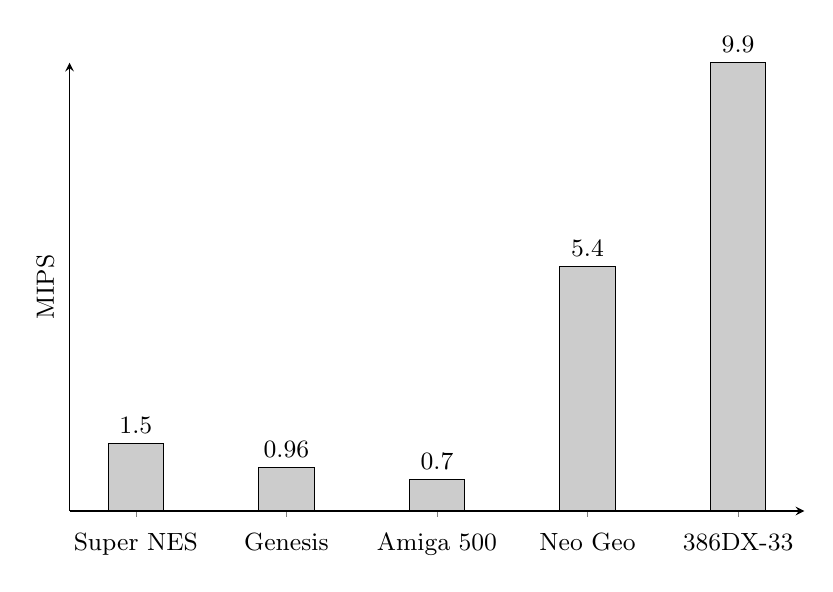
\begin{tikzpicture}[font=\small]
    \begin{axis}[
      width=0.9\textwidth,
      height=0.6\textwidth,
      ybar=6pt,
      bar width=20pt,
      ylabel={MIPS},
      ymin=0,
      ytick=\empty,
      xtick=data,
      axis x line=bottom,
      axis y line=left,
      enlarge x limits=0.11,
      symbolic x coords={Super NES,Genesis,Amiga 500,Neo Geo,386DX-33},
      xticklabel style={anchor=base,yshift=-\baselineskip},
      nodes near coords={\pgfmathprintnumber\pgfplotspointmeta}
    ]
      \addplot[fill=black!20,draw=black] coordinates {
        (Super NES,1.5)
        (Genesis,0.96)
        (Amiga 500,0.7)
        (Neo Geo,5.4)
        (386DX-33,9.9)
      };
    \end{axis}
   \end{tikzpicture}
   \caption{Game Console Vs PC.} \label{fig:game_console_vs_PC}
 \end{figure}
 
That would be omitting the fact that game console were designed around animation. They all featured coprocessors and Graphic Processing Unit relying on tile engines. Animating a sprite on the screen was just about to update its $(x,y)$ coordinates.\\
\\
On the contrary, IBM PC animation was next to impossible. Not even to mention many other obstacles related to the CPU and operating system backward compatibility.\\ This is where my admiration for Wolfenstein 3D started: id Software achieved the impossible by building a game engine able to not only workaround the many limitations of the machine but sometimes turn them into an advantage.\\
\\
I saw beauty in this ability to repurpose a machine to do something even the builder did not think was possible. It takes optimist, creativity, passion and dedication to be able to leave the safe harbour of the machine manual in order to Explore, Dream and Discover.\\
\\
This book tries to widen the window back on early 90s by not only describing the code but by also providing an overview of three pillars of game development:\\
\begin{itemize}
\item Hardware
\item People
\item Software
\end{itemize}

NOTE: What about a nice drawing instead ?

Additionally, a fourth part focuses on the post Wolfenstein 3D era.\\
\\
 \textbf{\underline{Disclaimer :}} The description that follows is technical and will most likely appeal to programmers. If you are more into the human aspect of game programming I would recommend instead to read David Kushner's chef d'oeuvre: "Masters of Doom: How Two Guys Created an Empire and Transformed Pop Culture".\\
 \\